\graphicspath{{./Chapters/CH5/Pictures/}}
\let\cleardoublepage\clearpage
\newcommand{\dfeq}[1]{\;\overset{\text{def}}{=}\;\label{eq:#1}}


\section{Harmonic Extraction Methodology}

This section develops a continuous narrative from standard three-phase modeling to harmonic-oriented synchronous frames used to render the characteristic 5th and 7th current components as constant (dc) quantities. Consider a surface-mounted PMSM (SPMSM) with non-salient inductances $L_d=L_q=L$, stator resistance $R_s$, permanent-magnet flux linkage $\psi_f$, and electrical rotor speed $\omega$. Let $(i_a,i_b,i_c)$ be the phase currents and $\theta$ the electrical angle. We first apply the Clarke transformation to obtain a stationary two-axis representation,

\begin{align}
i_a(t) &= I_1 \cos(\omega t+\theta_1) + I_5 \cos(5\omega t+\theta_5) + I_7 \cos(7\omega t+\theta_7), \label{eq:abc-a}\\
i_b(t) &= I_1 \cos\!\Big(\omega t-\tfrac{2\pi}{3}+\theta_1\Big)
        + I_5 \cos\!\Big(5\omega t+\tfrac{2\pi}{3}+\theta_5\Big)
        + I_7 \cos\!\Big(7\omega t-\tfrac{2\pi}{3}+\theta_7\Big), \label{eq:abc-b}\\
i_c(t) &= I_1 \cos\!\Big(\omega t+\tfrac{2\pi}{3}+\theta_1\Big)
        + I_5 \cos\!\Big(5\omega t-\tfrac{2\pi}{3}+\theta_5\Big)
        + I_7 \cos\!\Big(7\omega t+\tfrac{2\pi}{3}+\theta_7\Big). \label{eq:abc-c}
\end{align}

\begin{equation}
\begin{bmatrix} i_\alpha \\[2pt] i_\beta \end{bmatrix}
= \frac{2}{3}
\begin{bmatrix}
1 & -\tfrac{1}{2} & -\tfrac{1}{2} \\
0 & \tfrac{\sqrt{3}}{2} & -\tfrac{\sqrt{3}}{2}
\end{bmatrix}
\begin{bmatrix} i_a \\[2pt] i_b \\[2pt] i_c \end{bmatrix},
\label{eq:clarke}
\end{equation}
and then the Park transformation to rotate into the fundamental synchronous frame aligned with the rotor flux,
\begin{equation}
\begin{bmatrix} i_d \\[2pt] i_q \end{bmatrix}
=
\underbrace{\begin{bmatrix}
\cos\theta & \sin\theta \\
-\sin\theta & \cos\theta
\end{bmatrix}}_{R(\theta)}
\begin{bmatrix} i_\alpha \\[2pt] i_\beta \end{bmatrix},
\qquad
\psi_d = L\,i_d+\psi_f,\ \ \psi_q = L\,i_q .
\label{eq:park}
\end{equation}
In this fundamental $dq$ frame, the SPMSM voltage equations take the well-known form
\begin{equation}
\boxed{
\begin{aligned}
u_d &= R_s i_d + \frac{d\psi_d}{dt} - \omega\,\psi_q,\\
u_q &= R_s i_q + \frac{d\psi_q}{dt} + \omega\,\psi_d,
\end{aligned}}
\label{eq:fundamental-dq}
\end{equation}
and the electromagnetic torque reduces to $T_e=\tfrac{3}{2}p\,\psi_f\,i_q$ for the non-salient case (pole pairs $p$).

At this point the literature makes a crucial observation: if 5th and 7th current harmonics are present in the three-phase variables, they do \emph{not} become constant in the fundamental frame. Instead, after \eqref{eq:clarke}–\eqref{eq:park} their projections appear as sinusoids at $\mp 6\omega$ (respectively) superimposed on $(i_d,i_q)$. A convenient schematic is
\begin{equation}
\begin{bmatrix} i_d \\[2pt] i_q \end{bmatrix}
\approx
\begin{bmatrix} \bar i_d \\[2pt] \bar i_q \end{bmatrix}
+
I_5
\begin{bmatrix}
\cos(-6\omega t+\phi_5) \\[2pt]
\sin(-6\omega t+\phi_5)
\end{bmatrix}
+
I_7
\begin{bmatrix}
\cos(+6\omega t+\phi_7) \\[2pt]
\sin(+6\omega t+\phi_7)
\end{bmatrix}
+\cdots,
\label{eq:pm-6w}
\end{equation}
so in the fundamental frame the 5th “precesses” backward at $-6\omega$ and the 7th forward at $+6\omega$. This motivates the next step: define \emph{harmonic synchronous frames} that co-rotate with the targeted harmonic so that it becomes dc.

There are two equivalent ways to formalize these frames that are widely used and consistent if one keeps sign conventions straight. The first is to view them as additional rotations \emph{relative to} the fundamental frame. Because the 5th and 7th appear at $\mp 6\omega$ in \eqref{eq:pm-6w}, we rotate the fundamental axes by $\pm 6\omega t$ to freeze those oscillations:
\begin{equation}
\begin{bmatrix} i_{d5} \\[2pt] i_{q5} \end{bmatrix}
=
\underbrace{\begin{bmatrix}
\cos(-6\omega t) & \sin(-6\omega t)\\
-\sin(-6\omega t) & \cos(-6\omega t)
\end{bmatrix}}_{R(6\omega t)}
\begin{bmatrix} i_d \\[2pt] i_q \end{bmatrix},
\qquad
\begin{bmatrix} i_{d7} \\[2pt] i_{q7} \end{bmatrix}
=
\underbrace{\begin{bmatrix}
\cos(6\omega t) & \sin(6\omega t)\\
-\sin(6\omega t) & \cos(6\omega t)
\end{bmatrix}}_{R(-6\omega t)}
\begin{bmatrix} i_d \\[2pt] i_q \end{bmatrix}.
\label{eq:rel-6w-rotations}
\end{equation}

\begin{align}
i_{d\text{5}}
  &= I_1 \cos\!\big(6\omega t + \theta_1\big)
   + I_5 \cos\!\big(\theta_5\big)
   + I_7 \cos\!\big(12\omega t + \theta_7\big),\\
i_{q\text{5}}
  &= I_1 \sin\!\big(6\omega t + \theta_1\big)
   + I_5 \sin\!\big(\theta_5\big)
   + I_7 \sin\!\big(12\omega t + \theta_7\big).
\end{align}

Under \eqref{eq:rel-6w-rotations}, the 5th-order component becomes a dc vector in $(d_5,q_5)$ and the 7th-order component becomes a dc vector in $(d_7,q_7)$. The second, equivalent viewpoint is to define the harmonic-frame electrical angles directly with respect to the stator as $\theta_5=5\theta$ and $\theta_7=7\theta$, and then compose Clarke and Park using those angles. A compact direct map from phases to the 5th frame is
\begin{equation}
\begin{bmatrix}
i_{d5}\\[2pt] i_{q5}
\end{bmatrix}
= \frac{2}{3}
\begin{bmatrix}
\cos(5\theta) & \cos\!\big(5\theta-\tfrac{2\pi}{3}\big) & \cos\!\big(5\theta+\tfrac{2\pi}{3}\big)\\[3pt]
-\sin(5\theta) & -\sin\!\big(5\theta-\tfrac{2\pi}{3}\big) & -\sin\!\big(5\theta+\tfrac{2\pi}{3}\big)
\end{bmatrix}
\begin{bmatrix} i_a\\[2pt] i_b\\[2pt] i_c \end{bmatrix},
\label{eq:abc-d5q5}
\end{equation}
with the 7th-frame map obtained by replacing $5\theta$ with $7\theta$ and adjusting the signs consistently and applying DC low pass filter. In their own frames the targeted components are constant:
\begin{equation}
\boxed{
\begin{aligned}
i_{d5,h} &= I_5\cos\theta_5,\qquad &i_{q5,h} &= I_5\sin\theta_5,\\
i_{d7,h} &= I_7\cos\theta_7,\qquad &i_{q7,h} &= I_7\sin\theta_7,
\end{aligned}}
\label{eq:dc-in-harmonic-frames}
\end{equation}
where $(I_5,\theta_5)$ and $(I_7,\theta_7)$ are the amplitudes and initial phases of the 5th and 7th components.

\section{Harmonic Sources in PMSM: Inverter Non-Linearities Effects}
Nonlinearities in the inverter’s operation introduce significant distortions between the reference voltage commands and the actual output voltages. These nonlinearities degrade system performance, causing harmonic distortions, torque ripple, and instability in sensorless control schemes. The distortion voltage equations for the inverter nonlinearities in the synchronous reference frame (dq-axis) are expressed as follows:
\begin{equation}
\begin{bmatrix}
\delta v_d{}_{th} \\
\delta v_q{}_{th}
\end{bmatrix}
= 
3K_{abc}^{dq} \Lambda
\begin{bmatrix}
\text{sgn}(i_u) \\
\text{sgn}(i_v) \\
\text{sgn}(i_w)
\end{bmatrix}
+
K_{abc}^{dq} \frac{(R_{cc} + R_d)}{2}
\begin{bmatrix}
i_u \\
i_v \\
i_w
\end{bmatrix},
\label{eq:distortion_voltage}
\end{equation}

where $\Lambda$ is defined as follows:

\begin{equation}
\Lambda = \frac{(V_{dc} - V_{ce} + V_d)(T_{\text{dead}} + T_{\text{ON}} - T_{\text{OFF}})}{3T_s} + \frac{V_{\text{ce0}} + V_{\text{d0}}}{6},
\label{eq:Lambda}
\end{equation}
and $K_{abc}^{dq}$ is the following transformation matrix: 
\begin{equation}
K_{abc}^{dq} = 
\frac{2}{3}
\begin{pmatrix}
\cos\theta_e & \cos\left(\theta_e - \frac{2\pi}{3}\right) & \cos\left(\theta_e + \frac{2\pi}{3}\right) \\
-\sin\theta_e & -\sin\left(\theta_e - \frac{2\pi}{3}\right) & -\sin\left(\theta_e + \frac{2\pi}{3}\right)
\end{pmatrix}
\label{eq:transformation_matrix}
\end{equation}

\noindent By utilizing the distortion voltage equation (\ref{eq:distortion_voltage}) that capture the nonlinear behavior of power electronic inverters, the voltage dynamics in the(dq-axis) frame are updated as follows;

\begin{equation}
v_d - \delta v_{d\mathrm{th}} = R_s i_d + L_d \frac{d i_d}{d t} - \omega_e L_q i_q 
\label{eq:v_d_new}
\end{equation}
\begin{equation}
v_q - \delta v_{q\mathrm{th}} = R_s i_q + L_q \frac{d i_q}{d t} + \omega_e L_d i_d + \omega_e \lambda_f 
\label{eq:v_q_new}
\end{equation}

For conventional two-level VSIs employing pulse-width modulation (PWM), the dominant low-order harmonics in line currents are the $5^{\text{th}}$ and $7^{\text{th}}$ orders. These arise from Fourier decomposition of switched voltage waveforms. Therefore, most harmonic mitigation strategies focus on suppressing the $5^{\text{th}}$ and $7^{\text{th}}$ orders to minimize total harmonic distortion (THD) and improve power quality. The following presents the Fourier series-based analysis used to quantify the total harmonic distortion (THD) in the stator current in abc frame  

\begin{equation}
i_a = I_1 cos(\omega t+\theta_1) + I_5 cos(5\omega t+\theta_5) +  I_7 cos(7\omega t+\theta_7)
\end{equation}
\begin{equation}
i_b =I_1 cos(\omega t - 2 \pi/3 +\theta_1) + I_5 cos(5\omega t + 2 \pi/3 +\theta_5) + I_7 cos(7\omega t - 2\pi/3 +\theta_7)
\end{equation}
\begin{equation}
i_c = I_1 cos(\omega t + 2 \pi/3 +\theta_1) +I_5 cos(5\omega t - 2 \pi/3 +\theta_5) + I_7 cos(7\omega t + 2 \pi/3 +\theta_7)
\end{equation}

Then, the motor currents under odd harmonics in $d-q$ frame are;
\begin{equation}
i_d = I_1 cos(\theta_1) + I_5cos(-6\omega t + \theta_5) + I_7cos(6\omega t + \theta_7) = i_d{}_{1} + i_d{}_{5} + i_d{}_{7} 
\label{eq:id_total}
\end{equation}
\begin{equation}
i_q = I_1 sin(\theta_1) + I_5sin(-6\omega t + \theta_5) + I_7sin(6\omega t + \theta_7) = i_q{}_{1} + i_q{}_{5} + i_q{}_{7},
\label{eq:id_total}
\end{equation}



in which, the $5^{th}$ and $7^{th}$ harmonics in the abc frame appear in the fundamental \(dq\)-frame as sixth-order harmonics, but with opposite rotation directions: the 5th harmonic maps to a negative 6th harmonic (rotating backward at \(6\omega_e\)), while the 7th harmonic maps to a positive 6th harmonic (rotating forward at \(6\omega_e\)).

To deal with such harmonics in current signals, PMSMs are commonly controlled by proportional–integral (PI) control techniques augmented by harmonic compensators. The reference current is regulated and periodic disturbances are attenuated in order to suppress stator current harmonics and torque ripples. At low speeds, where inverter nonlinearities and back-electromotive force (EMF) harmonics have a more significant influence, these methods typically rely on additional resonant controllers tuned to specific harmonic orders or on feedforward voltage compensation to counteract known distortion sources. However, such approaches treat harmonic suppression indirectly, requiring separate loops or fixed-frequency compensators that may lose effectiveness under parameter variations, frequency drifts, or dynamic operating conditions. In contrast, MMPC can explicitly incorporate harmonic mitigation objectives into its cost function, enabling simultaneous current regulation and ripple suppression within a unified optimization framework. This direct inclusion allows MPC to adaptively address harmonic components across varying speeds and load conditions, offering improved performance and robustness compared to conventional cascaded compensator-based schemes.

\section{Hybrid Modulated Model Predictive Controller with Non-Linearities Harmonics Prediction}
The primary objective of this paper is to adopt the MMPC approach for operation at a fixed switching frequency, while also mitigating inverter nonlinearities through active compensation of low-order harmonics in the stator current of the PMSM. Due to the discrete nature of MMPC, we apply Euler’s forward discretization to \ref{eq:v_d_new} and \ref{eq:v_q_new}, resulting in the following expressions for the current dynamics:
\begin{equation}
\begin{aligned}
\begin{bmatrix}
i_d[k+1]\\
i_q[k+1]
\end{bmatrix}
&=
\left(1-\frac{R T_s}{L}\right)
\begin{bmatrix}
i_d[k]\\
i_q[k]
\end{bmatrix}
+
\frac{T_s}{L}
\begin{bmatrix}
v_d[k]-\delta v_d{}_{th}[k]\\
v_q[k]-\delta v_q{}_{th}[k]
\end{bmatrix} \\
&\quad
+ \omega T_s
\begin{bmatrix}
i_q[k]\\
-\,i_d[k]
\end{bmatrix}
+
\frac{\omega T_s}{L}
\begin{bmatrix}
0\\
\lambda_m
\end{bmatrix}
\end{aligned}
\label{eq:i_discrete}
\end{equation}
where  $T_s$ is the sampling time, $k$ is the sampling index, and $L=L_q=L_d$. By substituting the total current components from equations \ref{eq:id_total} \ref{eq:iq_total} into \ref{eq:i_discrete}, the expanded current dynamics become:

\begin{equation}
\begin{aligned}
\begin{bmatrix}
i_d{}_{1}[k+1] + i_d{}_{5}[k+1] + i_d{}_{7}[k+1]\\
i_q{}_{1}[k+1] + i_q{}_{5}[k+1] + i_q{}_{7}[k+1]
\end{bmatrix}
&=
\left(1-\frac{R T_s}{L}\right)
\begin{bmatrix}
i_d{}_{1}[k] + i_d{}_{5}[k] + i_d{}_{7}[k]\\
i_q{}_{1}[k] + i_q{}_{5}[k] + i_q{}_{7}[k]
\end{bmatrix}
+
\frac{T_s}{L}
\begin{bmatrix}
v_d[k] - \delta v_{dth}[k]\\
v_q[k] - \delta v_{qth}[k]
\end{bmatrix}\\
&\quad
+ \omega T_s
\begin{bmatrix}
i_q{}_{1}[k] + i_q{}_{5}[k] + i_q{}_{7}[k]\\
-\big(i_d{}_{1}[k] + i_d{}_{5}[k] + i_d{}_{7}[k]\big)
\end{bmatrix}
+
\frac{\omega T_s}{L}
\begin{bmatrix}
0\\
\lambda_m
\end{bmatrix}
\end{aligned}
\label{eq:expanded_current}
\end{equation}
Here, we can see that the stator currents in the \(dq\)-frame is expressed as a summation of the fundamental and dominant harmonic components, particularly the 5th and 7th. Consequently, the voltage-drop terms $\delta v_{d}{}_{th}, \delta v_{q}{}_{th}$ are decomposed based on the harmonic orders present in the current waveforms. This decomposition is given by:
\begin{equation}
\begin{aligned}
\begin{bmatrix}
\delta v_{dth}[k]\\
\delta v_{qth}[k]
\end{bmatrix}
=
\begin{bmatrix}
\delta v_d{}_{1}[k] + \delta v_d{}_{5}[k] + \delta v_d{}_{7}[k]\\
\delta v_q{}_{1}[k] + \delta v_q{}_{5}[k] + \delta v_q{}_{7}[k]
\end{bmatrix}
\end{aligned}
\end{equation}
A control technique such as MMPC allows the algorithm to predict and regulate each harmonic independently. This capability enables targeted suppression of unwanted current harmonics while maintaining accurate tracking of the fundamental current. Based on these objectives, the following cost function is defined for a single-step prediction:
\begin{equation}
\begin{aligned}
J(v_j) &=
Q_d \left\| i_{d1,v_j}[k+1] - i_d^{*} \right\|^2
+ Q_q \left\| i_{q1,v_j}[k+1] - i_q^{*} \right\|^2 \\
&\quad
+ \sum_{h} w_h \left(
\left\| i_{dh,v_j}[k+1] \right\|^2
+ \left\| i_{qh,v_j}[k+1] \right\|^2
\right)
\end{aligned}
\label{eq:cost_function_total}
\end{equation}
in which, \( i_{d1,v_i} \) and \( i_{q1,v_i} \) denote the fundamental predicted current resulting from applying the voltage vector \( v_i \). Here also, ${i_{d}^*,i_{q}^*}$ represent the reference currents provided by the outer control loop, and ${Q_d,Q_q, w_h}$ are positive  weights. The first two terms penalize the tracking error between the predicted and reference currents, while the third and forth terms impose penalties on the magnitudes of specific harmonic components, particularly the $5^{th}$ and $7^{th}$ harmonics, through their associated weights $w_h$. 
\par
The key challenge at this stage lies in accurately predicting the harmonic components of the current, denoted by $\left\lbrace i_{dh}[k+1], i_{qh}[k+1]\right\rbrace $, over the prediction horizon. Precise estimation of these harmonic currents is essential for correctly evaluating the cost function $J$. Therefore, the controller must incorporate an accurate model or estimation strategy capable of capturing the harmonic behavior of the motor current—particularly the 5\textsuperscript{th} and 7\textsuperscript{th} harmonics.

Here, we adopt the technique presented in \cite{harmonics_MSRF,MSRF_2016} for harmonic elimination using multiple synchronous rotating frames (MSRFs), in which current harmonics of different orders are transformed into their respective rotating reference frames. Using this MSRF-based approach, we derive the current dynamic equations to enable precise prediction of both the fundamental and harmonic components of the motor currents, which is crucial for achieving effective harmonic suppression in predictive control schemes.

To isolate and analyze specific harmonics, such as the 5\textsuperscript{th} and 7\textsuperscript{th}, the three-phase currents in the stationary abc-frame are first transformed into the fundamental $dq$ synchronous reference frame using the Clarke and Park transformations, denoted collectively by $T_{abc}$. Subsequently, an additional transformation is applied to shift from the fundamental $dq$ frame to the desired harmonic reference frames. For example, the transformation from the fundamental $dq$ frame to the fifth-order synchronous reference frame is given by:
\begin{align}
\begin{bmatrix}
i_d \\
i_q
\end{bmatrix}_{5\text{th-frame}}
&= T_{dq1}^{dq5} \cdot
\begin{bmatrix}
i_d \\
i_q
\end{bmatrix}
\end{align}
Thus, the complete transformation from the abc frame to the fifth-order synchronous $dq$ frame becomes:
\begin{equation}
\begin{bmatrix}
i_d \\
i_q
\end{bmatrix}_{5\text{th-frame}}
=
T_{dq1}^{dq5} \cdot T_{abc} \cdot
\begin{bmatrix}
i_a \\
i_b \\
i_c
\end{bmatrix}
\end{equation}
Similarly, the transformation to the seventh-order frame is:
\begin{equation}
\begin{bmatrix}
i_d \\
i_q
\end{bmatrix}_{7\text{th-frame}}
=
T_{dq1}^{dq7} \cdot T_{abc} \cdot
\begin{bmatrix}
i_a \\
i_b \\
i_c
\end{bmatrix}
\end{equation}
where
\begin{align}
T_{dq1}^{dq5}&=
\begin{bmatrix}
cos(-6\omega t)&sin(-6\omega t)\\
-sin(-6\omega t)&cos(-6\omega t)
\end{bmatrix}\\
T_{dq1}^{dq7}&=
\begin{bmatrix}
cos(6\omega t)&sin(6\omega t)\\
-sin(6\omega t)&cos(6\omega t)
\end{bmatrix}
\end{align}
This transformation occurs because the synchronous \(dq\)-frame rotates at the fundamental angular speed, effectively shifting harmonic orders by \(-1\) and reversing the sequence of negative-sequence harmonics. As a result, placing the $5^{th}$ and $7^{th}$ harmonic models in their respective \(\pm 6\omega_e\) rotating frames allows them to appear as DC quantities, greatly simplifying their prediction and suppression in the controller design. As we see in the following transformed frame, the current signals are projected onto the fifth-order synchronous frame, and their decomposition yields:
\begin{align}
i_{d,5\text{th-frame}} &= I_1 \cos(6\omega t + \theta_1) + I_5 \cos(\theta_5) + I_7 \cos(12\omega t + \theta_7) \\
i_{q,5\text{th-frame}} &= I_1 \sin(6\omega t + \theta_1) + I_5 \sin(\theta_5) + I_7 \sin(12\omega t + \theta_7)
\end{align}
where, the fifth-order harmonic appears as a DC component in this frame, and can be expressed as:
\begin{equation}
\begin{bmatrix}
i_{d5} \\
i_{q5}
\end{bmatrix}_{5th-frame}
= I_5
\begin{bmatrix}
\cos \theta_5 \\
\sin \theta_5
\end{bmatrix}
\end{equation}
Likewise, projecting the currents onto the seventh-order synchronous frame results in:
\begin{equation}
\begin{aligned}
i_{d,7\text{th-frame}} &= I_1 \cos(6\omega t - \theta_1) + I_5 \cos(12\omega t - \theta_5) + I_7 \cos(\theta_7) \\
i_{q,7\text{th-frame}} &= -I_1 \sin(6\omega t + \theta_1) - I_5 \sin(12\omega t - \theta_5) + I_7 \sin(\theta_7)
\end{aligned}
\end{equation}
in which, the seventh-order harmonic also manifests as a DC component:
\begin{equation}
\begin{bmatrix}
i_{d7} \\
i_{q7}
\end{bmatrix}_{7th-frame}
= I_7
\begin{bmatrix}
\cos \theta_7 \\
\sin \theta_7
\end{bmatrix}
\end{equation}
This property enables a low-pass filter to extract the DC components representing the fifth- and seventh-order harmonics in their respective rotating frames, which can then be directly used in the motor model equations to predict each harmonic.
% Predictive updates (fundamental, 5th-frame, 7th-frame)
Using the principle of superposition, the current dynamics are decomposed into three independent subsystems: the fundamental d–q frame for torque-producing currents, and the fifth- and seventh-harmonic d–q frames for the main harmonic distortions. Recalling \ref{eq:expanded_current}, each harmonic is predicted separately within its rotating reference frame using the d–q model equations as follows:
\begin{equation}
\begin{aligned}
\begin{bmatrix}
i_{d1}[k+1]\\
i_{q1}[k+1]
\end{bmatrix}
&=
\left(1 - \frac{R T_s}{L}\right)
\begin{bmatrix}
i_{d1}[k]\\
i_{q1}[k]
\end{bmatrix}
+
\frac{T_s}{L}
\begin{bmatrix}
v_d[k] - \delta v_{d1}[k]\\
v_q[k] - \delta v_{q1}[k]
\end{bmatrix}\\
&\quad
+ \omega T_s
\begin{bmatrix}
i_{q1}[k]\\
-\,i_{d1}[k]
\end{bmatrix}
+
\frac{\omega T_s}{L}
\begin{bmatrix}
0\\
\lambda_m
\end{bmatrix}
\end{aligned}
\label{eq:id1_predict}
\end{equation}

\begin{equation}
\begin{aligned}
\begin{bmatrix}
i_{d5}[k+1]\\
i_{q5}[k+1]
\end{bmatrix}_{\text{5th-frame}}
&=
\left(1 - \frac{R T_s}{L}\right)
\begin{bmatrix}
i_{d5}[k]\\
i_{q5}[k]
\end{bmatrix}_{\text{5th-frame}}
+
\frac{T_s}{L}
\begin{bmatrix}
-\,\delta v_{d5}[k]\\
-\,\delta v_{q5}[k]
\end{bmatrix}_{\text{5th-frame}}\\
&\quad
+ \omega T_s
\begin{bmatrix}
i_{q5}[k]\\
-\,i_{d5}[k]
\end{bmatrix}_{\text{5th-frame}}
\end{aligned}
\label{eq:id5_predict}
\end{equation}

\begin{equation}
\begin{aligned}
\begin{bmatrix}
i_{d7}[k+1]\\
i_{q7}[k+1]
\end{bmatrix}_{\text{7th-frame}}
&=
\left(1 - \frac{R T_s}{L}\right)
\begin{bmatrix}
i_{d7}[k]\\
i_{q7}[k]
\end{bmatrix}_{\text{7th-frame}}
+
\frac{T_s}{L}
\begin{bmatrix}
-\,\delta v_{d7}[k]\\
-\,\delta v_{q7}[k]
\end{bmatrix}_{\text{7th-frame}}\\
&\quad
+ \omega T_s
\begin{bmatrix}
i_{q7}[k]\\
-\,i_{d7}[k]
\end{bmatrix}_{\text{7th-frame}}
\end{aligned}
\label{eq:id7_predict}
\end{equation}

% How the current components at instant k are obtained

\begin{equation}
\begin{aligned}
\begin{bmatrix}
i_{d1}[k]\\
i_{q1}[k]
\end{bmatrix}
&=
\mathrm{LPF}
\begin{bmatrix}
i_d[k]\\
i_q[k]
\end{bmatrix},
\\[6pt]
\begin{bmatrix}
i_{d5}[k]\\
i_{q5}[k]
\end{bmatrix}_{\text{5th-frame}}
&=
\mathrm{LPF}\!\left(
T_{dq1}^{dq5}
\begin{bmatrix}
i_d[k]\\
i_q[k]
\end{bmatrix}
\right),
\\[6pt]
\begin{bmatrix}
i_{d7}[k]\\
i_{q7}[k]
\end{bmatrix}_{\text{7th-frame}}
&=
\mathrm{LPF}\!\left(
T_{dq1}^{dq7}
\begin{bmatrix}
i_d[k]\\
i_q[k]
\end{bmatrix}
\right)
\end{aligned}
\end{equation}

% Voltage-drop components

\begin{equation}
\begin{aligned}
\begin{bmatrix}
\delta v_{d1}[k]\\
\delta v_{q1}[k]
\end{bmatrix}
&=
\mathrm{LPF}
\begin{bmatrix}
\delta v_d{}_{th}[k]\\
\delta v_q{}_{th}[k]
\end{bmatrix},
\\[6pt]
\begin{bmatrix}
\delta v_{d5}[k]\\
\delta v_{q5}[k]
\end{bmatrix}_{\text{5th-frame}}
&=
\mathrm{LPF}\!\left(
T_{dq1}^{dq5}
\begin{bmatrix}
\delta v_d{}_{th}[k]\\
\delta v_q{}_{th}[k]
\end{bmatrix}
\right),
\\[6pt]
\begin{bmatrix}
\delta v_{d7}[k]\\
\delta v_{q7}[k]
\end{bmatrix}_{\text{7th-frame}}
&=
\mathrm{LPF}\!\left(
T_{dq1}^{dq7}
\begin{bmatrix}
\delta v_d{}_{th}[k]\\
\delta v_q{}_{th}[k]
\end{bmatrix}
\right)
\end{aligned}
\end{equation}

\begin{figure}[H]
\centering
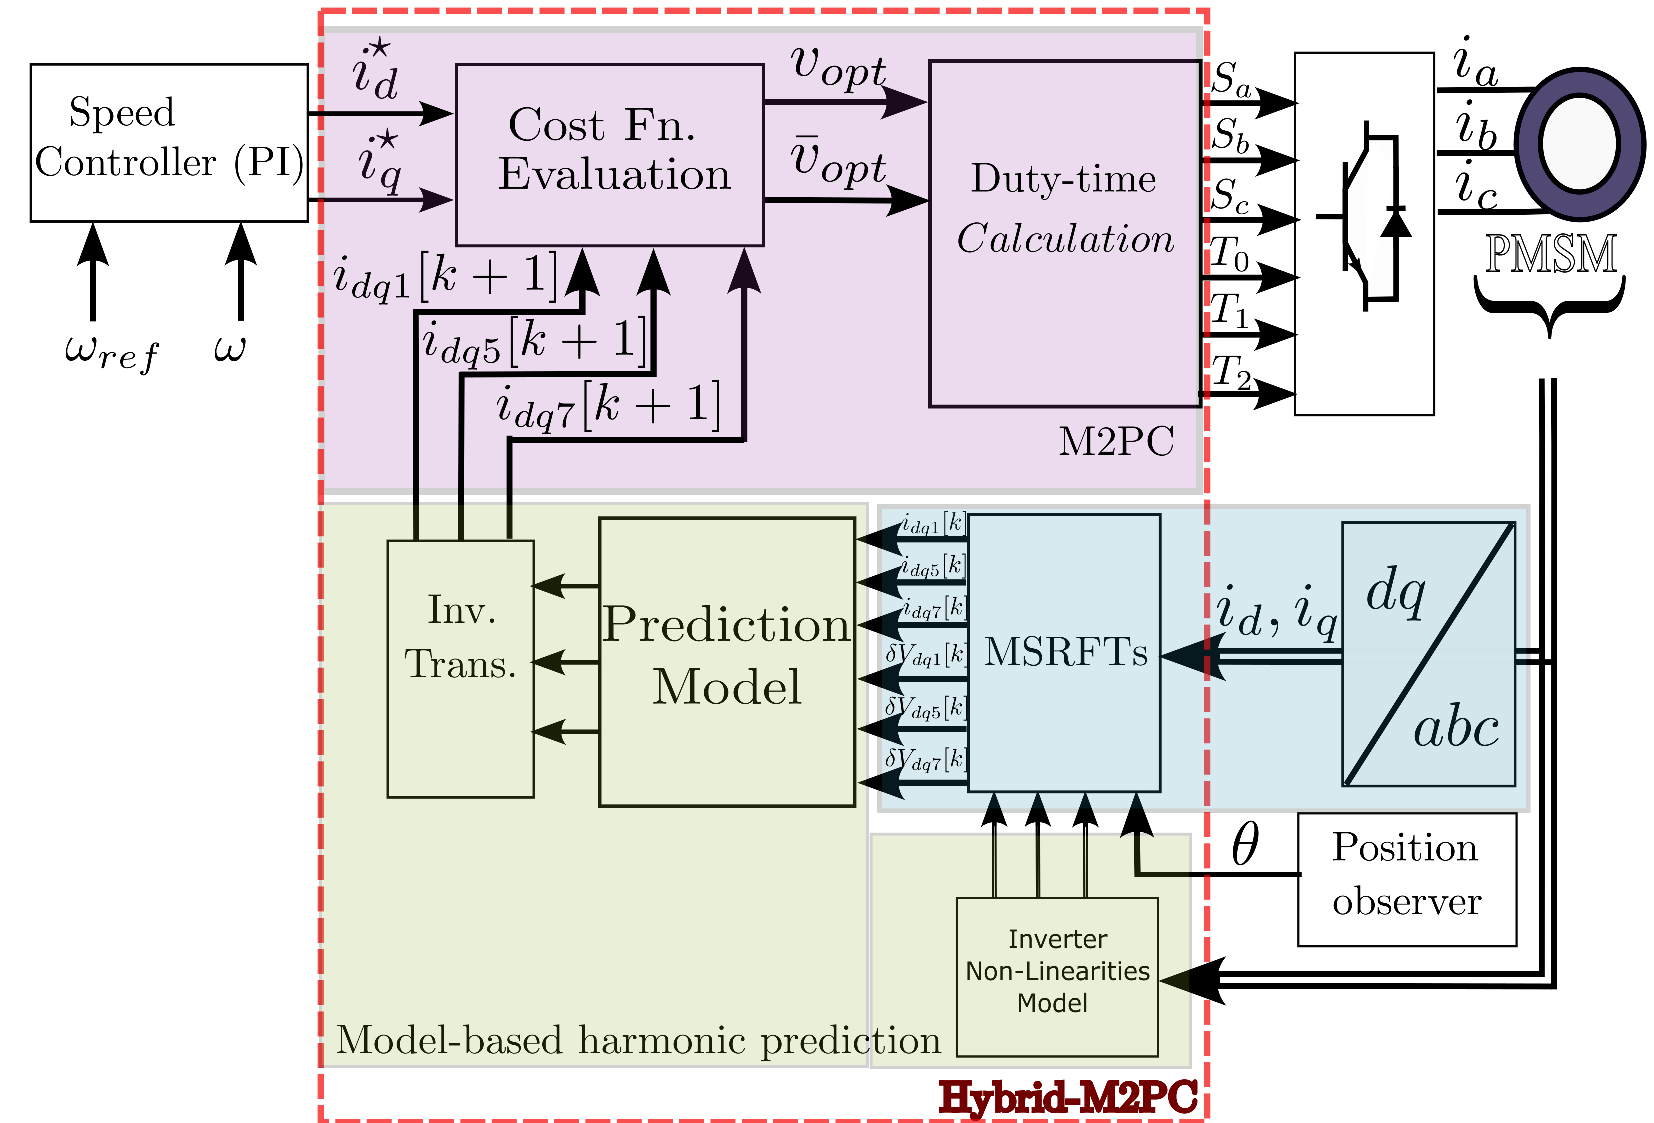
\includegraphics[width=\linewidth]{hybrid_MPC_updated}
\caption{Proposed Hybrid-MMPC scheme for PMSM drives, combining MMPC approach, and harmonic prediction in multiple synchronous rotating frames }
\label{fig:Proposed_M2PC}
\end{figure}

To realize optimal voltage application within a single sampling period, the control strategy involves selecting two active voltage vectors, \( \mathbf{v}_{\text{opt}} \) and \( \mathbf{v}'_{\text{opt}} \), along with the zero vector \( \mathbf{v}_0 \). The sub-indices 0, 1, and 2 correspond to the zero vector \( \mathbf{v}_0 \), the optimal voltage vector \( \mathbf{v}_{\text{opt}} \), and the second optimal vector \( \mathbf{v}'_{\text{opt}} \), respectively, selected based on minimizing the cost function defined in~\eqref{eq:cost_function_total}. These vectors are time-modulated during the sampling interval such that their weighted average closely approximates the desired voltage, thereby reducing the current tracking error to nearly zero. the following equations clarify this objective;

\begin{align}
\sum_{j=0}^{2} T_j\, i_{d,v_j}[k+1] &= T_s\, i_d^{*} \label{eq:modulated_mpc_constraints_1}\\
\sum_{j=0}^{2} T_j\, i_{q,v_j}[k+1] &= T_s\, i_q^{*} \label{eq:modulated_mpc_constraints_2}
\end{align}
where
\begin{equation}
\sum_{j=0}^{2} T_j = T_s
\label{eq:modulated_mpc_constraints_3}
\end{equation}
Here, equations~\eqref{eq:modulated_mpc_constraints_1}–\eqref{eq:modulated_mpc_constraints_3} define a linear system of equations used to determine the optimal duty times \( T_0, T_1, T_2 \) associated with the selected voltage vectors \( v_j \). These equations ensure that the weighted sum of the resulting currents aligns with the desired current reference \( (i_d^*, i_q^*) \) over one sampling interval \( T_s \), while also satisfying the time constraint on vector modulation. The duty times \( T_0, T_1, T_2 \) can be computed by solving the following linear system:
\begin{equation}
\begin{bmatrix}
i_{d,v_0}[k+1] & i_{d,v_1}[k+1] & i_{d,v_2}[k+1] \\
i_{q,v_0}[k+1] & i_{q,v_1}[k+1]  & i_{q,v_2}[k+1]  \\
1        & 1        & 1
\end{bmatrix}
\begin{bmatrix}
T_0 \\ T_1 \\ T_2
\end{bmatrix}
=
\begin{bmatrix}
T_s i_d^* \\ T_s i_q^* \\ T_s
\end{bmatrix}
\label{eq:duty_time_solution}
\end{equation}

\noindent
Thus, the optimal duty vector is computed as:
\begin{equation}
\begin{bmatrix}
T_0 \\ T_1 \\ T_2
\end{bmatrix}
=
\begin{bmatrix}
i_{d,v_0}[k+1] & i_{d,v_1}[k+1] & i_{d,v_2}[k+1] \\
i_{q,v_0}[k+1] & i_{q,v_1}[k+1]  & i_{q,v_2}[k+1]  \\
1        & 1        & 1
\end{bmatrix}^{-1}
\begin{bmatrix}
T_s i_d^* \\ T_s i_q^* \\ T_s
\end{bmatrix}
\label{eq:duty_time_closed_form}
\end{equation}

\section{Control Algorithm Summary}
% Harmonic Current Prediction and Compensation — plain enumerate (no algorithm packages)

\begin{enumerate}
  \item Measure the phase currents and transform them to the fundamental $d$–$q$ frame.

  \item Obtain the separated components
  $
  \begin{bmatrix} i_{d1}[k]\\ i_{q1}[k]\end{bmatrix},\ 
  \begin{bmatrix} i_{d5}[k]\\ i_{q5}[k]\end{bmatrix}_{\text{5th-frame}},\ 
  \begin{bmatrix} i_{d7}[k]\\ i_{q7}[k]\end{bmatrix}_{\text{7th-frame}}.
  $

  \item Compute the one-step-ahead nominal prediction (fundamental frame):
  \[
  \begin{bmatrix} i_{d1}[k+1]\\ i_{q1}[k+1]\end{bmatrix}
  =
  \left(1-\frac{R T_s}{L}\right)
  \begin{bmatrix} i_{d1}[k]\\ i_{q1}[k]\end{bmatrix}
  + \frac{T_s}{L}\begin{bmatrix} v_d[k]\\ v_q[k]\end{bmatrix}
  + \omega T_s \begin{bmatrix} i_{q1}[k]\\ -\,i_{d1}[k]\end{bmatrix}
  + \frac{\omega T_s}{L}\begin{bmatrix} 0\\ \lambda_m\end{bmatrix}.
  \]

  \item Using the predicted currents from Step 3, compute the nonlinear voltage drop $\delta v_{\mathrm{th}}$ from (\ref{eq:distortion_voltage}).

  \item Form the decomposed voltage-drop components
  $
  \begin{bmatrix}\delta v_{d1}[k]\\ \delta v_{q1}[k]\end{bmatrix},\
  \begin{bmatrix}\delta v_{d5}[k]\\ \delta v_{q5}[k]\end{bmatrix}_{\text{5th-frame}},\
  \begin{bmatrix}\delta v_{d7}[k]\\ \delta v_{q7}[k]\end{bmatrix}_{\text{7th-frame}}.
  $

  \item Predict currents in the 5th and 7th frames using (\ref{eq:id5_predict}) and (\ref{eq:id7_predict}).

  \item Transform the predicted harmonic-frame currents back to the fundamental frame:
  \[
  \begin{bmatrix} i_{d5}[k+1]\\ i_{q5}[k+1] \end{bmatrix}
  = \left(T_{dq1}^{dq5}\right)^{-1}
    \begin{bmatrix} i_{d5h}[k+1]\\ i_{q5h}[k+1]\end{bmatrix},
  \qquad
  \begin{bmatrix} i_{d7}[k+1]\\ i_{q7}[k+1] \end{bmatrix}
  = \left(T_{dq1}^{dq7}\right)^{-1}
    \begin{bmatrix} i_{d7h}[k+1]\\ i_{q7h}[k+1]\end{bmatrix}.
  \]

  \item Evaluate the cost function $J(v_i)$ using the predicted currents.

  \item Store the pair $(J, v_i)$ for later selection.

  \item Repeat Steps 1–9 for $i=0,\ldots,7$.

  \item Select the optimal and sub-optimal switching vectors $(v_1, v_2)$ that yield the minimum $J$.

  \item Compute the duty times $T_0, T_1, T_2$ using (\ref{eq:duty_time_closed_form}).
\end{enumerate}
\section{Simulation Modeling}
This section validates the complete drive model and controllers through a focused suite of studies: (i) steady-state operation to verify ripple, losses, and harmonic content; (ii) low-speed operation to probe back-EMF limits and non-idealities; (iii)  dynamic performance under speed/current steps; (iv) parameter variation to gauge robustness against model mismatch; and (v) load variation to assess torque disturbance rejection.
\subsection{Steady State Operation}
At 1000 rpm with dead time and device drops enabled, the MMPC augmented with harmonic extraction sustains tight regulation and further reduces ripple relative to the basic MMPC. At low load (10\% rated torque, \(0.3~\mathrm{N\,m}\)) the phase-current THD drops to 6.5\% (vs.\ \(\sim\)8\% basic), see Fig.~\ref{fig:M2PCNL_HE_1000rpm_low}; at medium load (50\% rated torque, \(1.75~\mathrm{N\,m}\)) it falls to 0.8\% (vs.\ \(\sim\)2\% basic), see Fig.~\ref{fig:M2PCNL_HE_1000rpm_med}. These improvements—about \(1.5\) and \(1.2\) percentage points, respectively—reflect extraction/cancellation of the dominant low-order odd harmonics injected by non-ideal switching, while preserving fixed-frequency SVM actuation and excellent steady-state speed regulation.
% Requires in preamble:
% \usepackage{graphicx}
% \usepackage{subcaption}

\begin{figure}[H]
  \centering
  % --- (a) Low load with harmonic extraction ---
  \begin{subfigure}{0.485\textwidth}
    \centering
    % Replace with your exported plot/image
    
\includegraphics[width=\linewidth]{MPCMidSpeedLowLoadSteadyState}
    \caption{Low load: \(T=0.3~\mathrm{N\,m}\). THD \(=6.5\%\) (vs.\ \(8\%\) basic).}
    \label{fig:M2PCNL_HE_1000rpm_low}
  \end{subfigure}\hfill
  % --- (b) Medium load with harmonic extraction ---
  \begin{subfigure}{0.485\textwidth}
    \centering
    % Replace with your exported plot/image
    
\includegraphics[width=\linewidth]{MPCMidSpeedMidLoadSteadyState}
    \caption{Medium load: \(T=1.75~\mathrm{N\,m}\). THD \(=0.8\%\) (vs.\ \(2\%\) basic).}
    \label{fig:M2PCNL_HE_1000rpm_med}
  \end{subfigure}

  \caption{MMPC with harmonic extraction at 50\% rated speed (1000 rpm) under inverter non-linearities (dead time, device drops). Each panel shows \(i_{dq}\), phase currents, and THD.}
  \label{fig:M2PCNL_HE_1000rpm}
\end{figure}


\subsection{Low Speed Operation}

\begin{figure}[H]
  \centering

  % --- Row 1: 5% rated speed (100 rpm) ---
  \begin{subfigure}{0.4\textwidth}
    \centering
    % Replace with your exported plot/image
    
\includegraphics[width=\linewidth]{./MPCSteadyStateLowLoad100Rpm}
    \caption{5\% speed (100 rpm), low load \(T=0.3~\mathrm{N\,m}\); THD \(=2.8\%\).}
    \label{fig:M2PCNL_HE_100rpm_low}
  \end{subfigure}\hfill
  \begin{subfigure}{0.4\textwidth}
    \centering
    % Replace with your exported plot/image
    
\includegraphics[width=\linewidth]{./MPCSteadyStateHighLoad100Rpm}
    \caption{5\% speed (100 rpm), rated load \(T=3.5~\mathrm{N\,m}\); THD \(=0.8\%\).}
    \label{fig:M2PCNL_HE_100rpm_high}
  \end{subfigure}

  \vspace{0.6em}

  % --- Row 2: 10% rated speed (200 rpm) ---
  \begin{subfigure}{0.4\textwidth}
    \centering
    % Replace with your exported plot/image
    
\includegraphics[width=\linewidth]{./MPCSteadyStateLowLoad200Rpm}
    \caption{10\% speed (200 rpm), low load \(T=0.5~\mathrm{N\,m}\); THD \(=2.9\%\).}
    \label{fig:M2PCNL_HE_200rpm_low}
  \end{subfigure}\hfill
  \begin{subfigure}{0.4\textwidth}
    \centering
    % Replace with your exported plot/image
    
\includegraphics[width=\linewidth]{./MPCSteadyStateHighLoad200Rpm}
    \caption{10\% speed (200 rpm), rated load \(T=3.5~\mathrm{N\,m}\); THD \(=0.6\%\).}
    \label{fig:M2PCNL_HE_200rpm_high}
  \end{subfigure}

  \caption{Proposed MMPC-HE at low speeds under inverter non-linearities (dead time, device drops). Each panel shows \(i_{dq}\), phase currents, and THD.}
  \label{fig:M2PCNL_HE_low_speeds}
\end{figure}
With dead time and device drops enabled, the MMPC with harmonic extraction maintains stable sensorless operation and markedly reduces distortion at very low speeds. At 5\% rated (100~rpm), the phase-current THD is 2.8\% at low load (\(0.3~\mathrm{N\,m}\); see Fig.~\ref{fig:M2PCNL_HE_100rpm_low}) versus \(\sim\)6.9\% for the MMPC, and 0.8\% at rated load (\(3.5~\mathrm{N\,m}\); see Fig.~\ref{fig:M2PCNL_HE_100rpm_high}) versus \(\sim\)1.1\%. At 10\% rated (200~rpm), THD is 2.9\% at low load (\(0.5~\mathrm{N\,m}\); see Fig.~\ref{fig:M2PCNL_HE_200rpm_low}) compared with \(\sim\)6.6\% for the basic scheme, and 0.6\% at rated load (\(3.5~\mathrm{N\,m}\); see Fig.~\ref{fig:M2PCNL_HE_200rpm_high}) compared with \(\sim\)1.1\%. These gains arise from extracting/cancelling dominant low-order distortion components injected by non-ideal switching while preserving fixed-frequency SVM actuation and accurate one-step prediction, yielding the best low-speed THD among all controllers studied.

\subsection{Dynamic Performance}
With dead time and device drops enabled, the MMPC-HE tracks speed commands across the 10–50\% band (100–1000~rpm) cleanly at both load extremes—low load (\(0.3~\mathrm{N\,m}\); see Fig.~\ref{fig:M2PCNL_HE_Dyn_100to1000_low}) and rated load (\(3.5~\mathrm{N\,m}\); see Fig.~\ref{fig:M2PCNL_HE_Dyn_100to1000_rated}). In all transitions the measured speed follows the reference with overshoot \(\mathbf{<10\%}\) and negligible steady-state error; \(i_q\) steps proportionally, and the phase currents remain notably smooth, yielding lower torque ripple than all other controllers. Importantly, the harmonic–extraction stage—implemented as selective cancellation of low-order distortion in the commanded average voltage—does not alter the closed-loop dynamics: rise/settling times and damping are essentially unchanged from the baseline MMPC.
% Requires in preamble:
% \usepackage{graphicx}
% \usepackage{subcaption}

\begin{figure}[H]
  \centering
  % --- (a) Low load ---
  \begin{subfigure}{0.485\textwidth}
    \centering
    % Replace with your exported plot/image
    
\includegraphics[width=\linewidth]{MPCDynamicResponseLowLoad}
    \caption{Low load: \(T=0.3~\mathrm{N\,m}\). Overshoot \(<10\%\); smooth \(i_q\)/phase currents; very low torque ripple.}
    \label{fig:M2PCNL_HE_Dyn_100to1000_low}
  \end{subfigure}\hfill
  % --- (b) Rated load ---
  \begin{subfigure}{0.485\textwidth}
    \centering
    % Replace with your exported plot/image
    
\includegraphics[width=\linewidth]{MPCDynamicResponseHighLoad}
    \caption{Rated load: \(T=3.5~\mathrm{N\,m}\). Overshoot \(<10\%\); damping and settling comparable to baseline MPC.}
    \label{fig:M2PCNL_HE_Dyn_100to1000_rated}
  \end{subfigure}

  \caption{Dynamic performance of MMPC-HE under inverter non-linearities
  (dead time, device drops) for speed changes within the \(10\%\!\to\!50\%\) rated band (100–1000 rpm). Each panel shows
  command vs.\ speed, \(i_q\), and phase currents.}
  \label{fig:M2PCNL_HE_Dyn_100to1000}
\end{figure}

\subsection{Parameter Variation}
At 5\% rated speed (100~rpm) with dead time and device drops enabled, the proposed controller was stressed with a biased prediction model (\(R_s{+}25\%\), \(L_{d,q}{-}25\%\)). As shown in Fig.~\ref{fig:M2PCNL_HE_ParamVariation}, the phase-current THD is 4.6\%, notably lower than the 8.7\% obtained by the \emph{basic} MMPC under the same bias (cf. Fig.~\ref{fig:M2PCNL_ParamVariation}). The fixed-frequency SVM and per-sample voltage optimization preserve the closed-loop cutoff, but the harmonic-extraction stage is model-referenced; the parameter bias shifts the phase/amplitude of the dominant low-order distortion, so the template is imperfect and cancellation is incomplete—hence reduced (but nonzero) residual harmonics.

% Requires in preamble:
% \usepackage{graphicx}

\begin{figure}[h]
  \centering
  % Replace with your exported composite plot (e.g., speed, dq currents, phase currents, THD)
  
\includegraphics[width=0.7\linewidth]{MPCParameterVariation}
  \caption{Proposed MMPC-HE under parameter variation
  at 5\% rated speed (100 rpm) with inverter non-linearities (dead time, device drops).
  The prediction model is biased with \(R_s{+}25\%\) and \(L_{d,q}{-}25\%\).
  The composite plot reports \(d\)- and \(q\)-axis currents, phase currents, and the THD result.}
  \label{fig:M2PCNL_HE_ParamVariation}
\end{figure}

\subsection{Load Variation}
With dead time and device drops enabled, the motor was held at 1000 rpm while the load torque stepped from 10\% to 100\% of rated in 20\% increments. As shown in Fig.~\ref{fig:M2PCNL_HE_LoadVariation}, the proposed MMPC with harmonic extraction maintains the commanded speed without droop; \(i_q\) increases in clean, proportional steps, and the phase currents remain smooth. Transient metrics—rise time, settling, and damping—are essentially unchanged relative to the baseline MMPC (cf. Fig.~\ref{fig:M2PCNL_LoadVariation}), confirming that the harmonic-extraction stage does not penalize dynamics while preserving (and slightly improving) ripple performance under load changes.

% Requires in preamble:
% \usepackage{graphicx}

\begin{figure}[H]
  \centering
  % Replace with your exported composite plot:
  % (left) speed response, (middle) q-axis current, (right) phase currents
  
\includegraphics[width=0.6\linewidth]{MPCLoadVariation}
  \caption{Proposed MMPC-HE under load variation at 50\% rated speed
  (1000 rpm) with inverter non-linearities (dead time, device drops). The composite figure shows motor speed,
  \(i_q\), and phase currents during torque steps from 10\% to 100\% of rated in 20\% increments.}
  \label{fig:M2PCNL_HE_LoadVariation}
\end{figure}

\section{Experimental Validation}
This section presents the experimental validation of the proposed (MMPC-HE) for mitigating inverter non-linearities in a motor drive system. The experiments assess steady-state and dynamic performance under low-load conditions at a low speed and a higher speed. The MMPC-HE is compared against (MMPC), and a conventional proportional-integral (PI) controller at the higher speed, as the PI controller was unstable at the low speed due to its sensitivity to non-linearities. Performance is evaluated using phase current waveforms, d-q axis currents ($i_d$ and $i_q$), and total harmonic distortion (THD) to quantify harmonic suppression and control accuracy.

The experiments were conducted on a \SI{1}{kW} PMSM test bench, powered by a three-phase voltage source inverter (VSI) operating at a switching frequency of \SI{10}{kHz}. A generator was coupled to the motor to apply controlled load conditions, emphasizing inverter-induced non-linearities. The control algorithms were implemented on a Texas Instruments C2000 digital signal processor (DSP) with a control cycle update of \SI{100}{\micro\second}. Phase current measurements were obtained using two high-precision Hall-effect sensors.

Performance metrics include phase current waveforms, d-q axis currents ($i_d$ and $i_q$), and total harmonic distortion (THD).
\subsection{Steady-State Performance}
% Outlining the steady-state test design and evaluation metrics
Steady-state tests were conducted at the low and higher speeds to evaluate harmonic suppression and control accuracy at low loads, 10\% of the rated load. At the low speed, MMPC-HE and MMPC were compared, while at the higher speed, the PI controller was included as a baseline. The evaluation metrics included phase current waveforms to visually inspect harmonic distortions, d-q axis currents to assess control accuracy in the synchronous reference frame, and THD, defined as the percentage ratio of harmonic amplitudes to the fundamental component. 

% Presenting and analyzing steady-state results
The steady-state results are summarized in Table~\ref{tab:steady_state_results} and illustrated in Figures~\ref{fig:steady_state_100rpm}and~\ref{fig:steady_state_200rpm}. At the low speed, MMPC-HE exhibited significantly lower THD compared to MMPC, indicating effective harmonic suppression. At the higher speed, MMPC-HE outperformed both MMPC and the PI controller in THD reduction. Phase current waveforms for MMPC-HE showed smoother profiles with minimal distortions, and d-q axis currents displayed reduced oscillations, confirming superior tracking accuracy. The THD improvement of MMPC-HE was statistically significant, MMPC-HE demonstrated enhanced harmonic suppression under similar conditions.

\begin{table}[h]
\centering
\caption{Steady-State THD Comparison at Low Load}
\label{tab:steady_state_results}
\begin{tabular}{l c c}
\hline
Method & THD (100 RPM) & THD (200 RPM) \\
\hline
PI Controller & -- & 12.3\% \\
MMPC & 5.2\% & 3.1\% \\
MMPC-HE (Proposed) & 4.2\% & 2.3\% \\
\hline
\end{tabular}
\end{table}

\begin{figure}[H]
\centering
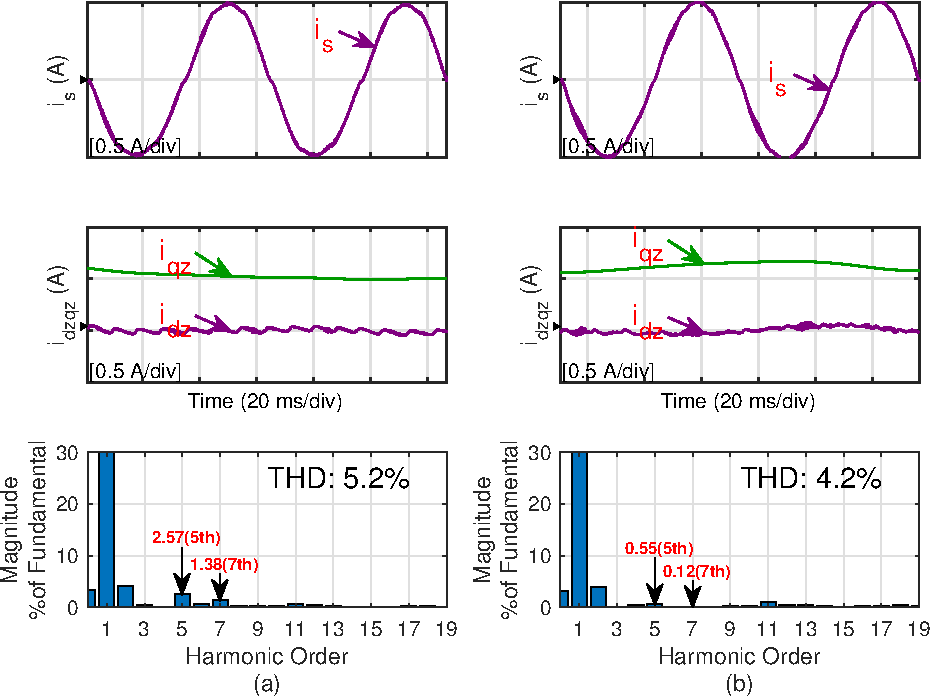
\includegraphics[width=0.8\textwidth]{./SteadyState100Rpm.pdf}
\caption{Experimental results of stator currents, $dz-qz$ axes currents, THD in low-speed (100 RPM) light load condition. (a) MMPC, (b) MMPC-HE.}
\label{fig:steady_state_100rpm}
\end{figure}

\begin{figure}
\centering
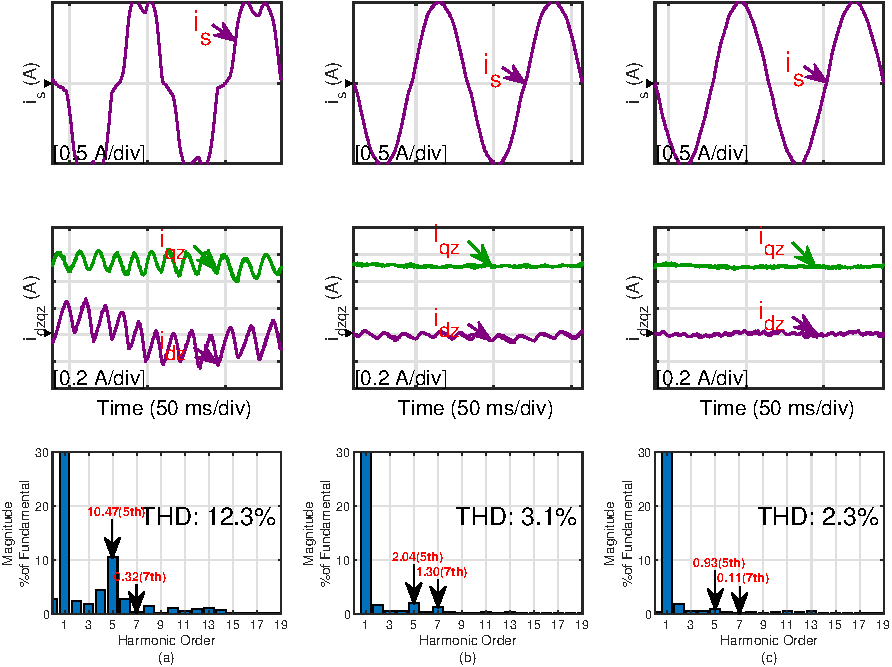
\includegraphics[width=0.8\textwidth]{./SteadyState200Rpm.pdf}
\caption{Experimental results of stator currents, $dz-qz$ axes currents, THD in low-speed (200 RPM) light load condition. (a) PI-Controller (b) MMPC, (c) MMPC-HE.}
\label{fig:steady_state_200rpm}
\end{figure}

\begin{figure}[H]
\centering
\includegraphics[width=8cm]{./hardware_setup}
\caption{Hardware setup}
\label{fig:hardware_setup}
\end{figure}

\subsection{Dynamic Response}
Dynamic response tests assessed the transient performance of the control methods under two speed step conditions. The first test evaluated MMPC-HE alone for a speed step from \SI{100}{rpm} to \SI{500}{rpm} to assess its transient response at higher speeds. The second test evaluated MMPC-HE, MMPC, and the PI controller for a speed step from \SI{500}{rpm} to \SI{100}{rpm} to compare their performance at lower speeds. The metrics included speed response, defined as the time taken for the motor speed to stabilize within a small percentage of the target speed, overshoot in the quadrature-axis current ($i_q$), and stator current waveforms to assess transient harmonic content.

The dynamic response results are presented in Figures~\ref{fig:DynamicHE_response}, and \ref{fig:DynamicAll_response}. For the speed step from \SI{100}{rpm} to \SI{500}{rpm}, MMPC-HE exhibited rapid speed response, minimal $i_q$ overshoot, and stator current waveforms with low harmonic distortion, demonstrating robust transient performance. For the speed step from \SI{500}{rpm} to \SI{100}{rpm}, MMPC-HE achieved a speed response comparable to MMPC-NHE but with significantly reduced $i_q$ undershoot, indicating stable control and rapid response unaffected by the harmonic extraction and elimination correction factor. while the PI controller exhibited an unstable response due to its inability to mitigate non-linearities at low speeds, resulting in pronounced stator current distortions.

\begin{figure}[H]
\centering
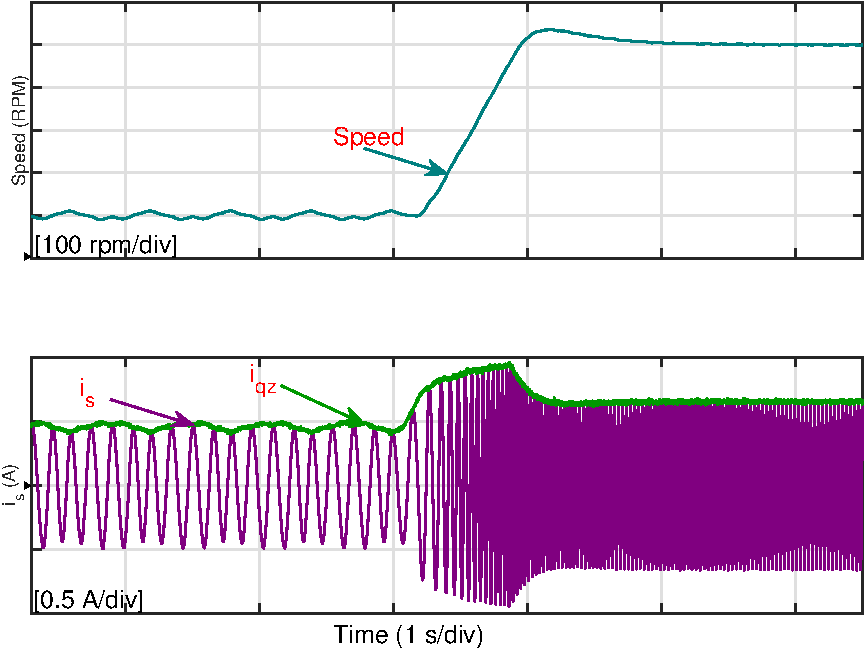
\includegraphics[width=0.6\textwidth]{./DynamicResponseHE.pdf}
\caption{Experimental results of stator currents, $qz$ axis current, and the speed response.}
\label{fig:DynamicHE_response}
\end{figure}

\begin{figure}[H]
\centering
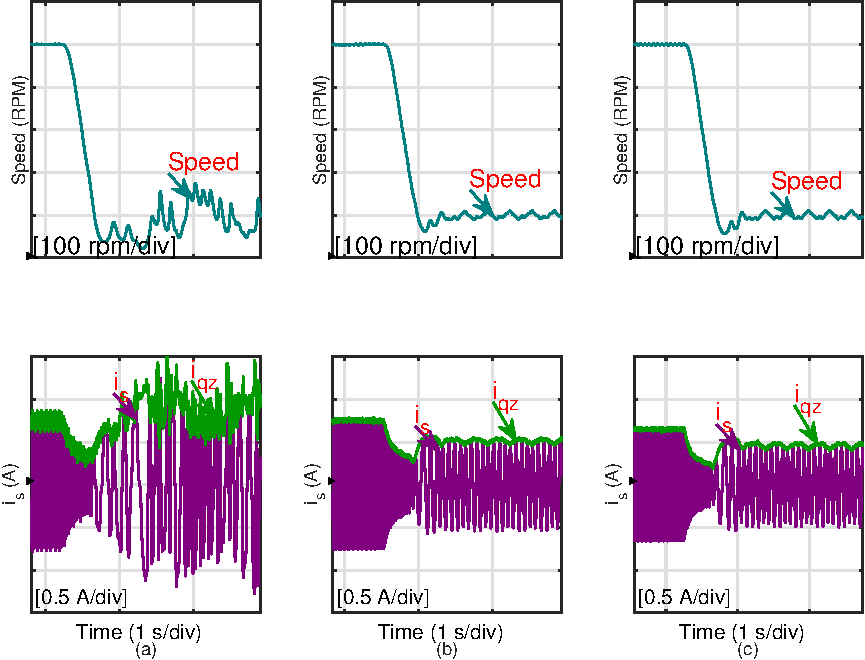
\includegraphics[width=0.6\textwidth]{./DynamicResponseAll.pdf}
\caption{Experimental results of stator currents, $qz$ axis current, and the speed response. (a) PI-Controller (b) MMPC, (c) MMPC-HE.}
\label{fig:DynamicAll_response}
\end{figure}


\subsection{Parameter Variation}
To evaluate the robustness of the proposed controller, a motor parameter variation test was conducted. In this test, key parameters of the permanent magnet synchronous motor (PMSM)—such as stator resistance, and inductance—were intentionally varied within a predefined range to emulate real-world operating conditions, including temperature fluctuations, aging effects, and manufacturing tolerances. The controller’s performance was assessed under these parameter deviations by monitoring current regulation, and overall stability. This procedure allowed for quantifying the sensitivity of the control algorithm to parameter uncertainties and verifying its capability to maintain reliable operation despite motor model mismatches.

The results of the motor parameter variation test, illustrated in Figure \ref{fig:ParameterVariation}, highlight the superior performance of the proposed hybrid modulated model predictive current controller in terms of current quality. When subjected to parameter deviations, the conventional PI current controller exhibited a significant degradation in performance, with the total harmonic distortion (THD) increasing by approximately 7\%. In comparison, the modulated model predictive current controller demonstrated improved robustness, showing only a 0.6\% increase in THD under the same conditions. The proposed hybrid approach achieved the best performance, limiting the THD increase to just 0.2\%, thereby confirming its enhanced capability to handle parameter variations while maintaining high-quality current waveforms

\begin{figure}[H]
\centering

\includegraphics[width=0.6\textwidth]{./ParameterVariation.pdf}
\caption{Experimental results of stator currents, $dz-qz$ axes currents, THD in low-speed (200 RPM) light load condition with motor parameters Variation. (a) PI-Controller (b) MMPC, (c) MMPC-HE.}
\label{fig:ParameterVariation}
\end{figure}

\subsection{CPU Load Consumption}
% Outlining the CPU load test design and evaluation metrics
CPU load consumption tests were conducted to evaluate the computational burden of the control methods, particularly due to the extensive use of sine and cosine operations in MMPC-HE. The tests measured the execution time of each control algorithm on the C2000 DSP under steady-state conditions at the low and higher speeds. The evaluation metric was the percentage of the \SI{100}{\micro\second} control cycle consumed by the algorithm, reflecting the computational load relative to the available processing time.

% Presenting and analyzing CPU load consumption results
The CPU load consumption results are summarized in Table~\ref{tab:cpu_load_results}. At both the low and higher steady state speeds, MMPC-HE exhibited a higher computational load compared to MMPC and the PI controller, attributed to the additional sine and cosine operations required for harmonic extraction and elimination. However, the execution time of MMPC-HE remained within the \SI{100}{\micro\second} control cycle, indicating feasibility for real-time implementation on the C2000 DSP. In contrast, MMPC and the PI controller required less computational time, with the PI controller showing the lowest CPU load due to its simpler control structure. These results highlight a trade-off between the enhanced harmonic suppression of MMPC-HE and its increased computational demand, which warrants further optimization in future work.

\begin{table}[h]
\centering
\caption{CPU Load Consumption Comparison}
\label{tab:cpu_load_results}
\begin{tabular}{l c}
\hline
Method & CPU Load (\%) \\
\hline
PI Controller & 3.5  \\
MMPC & 34\\
MMPC-HE (Proposed) & 45 \\
\hline
\end{tabular}
\end{table}

\begin{figure}[htbp]
    \centering
    \begin{minipage}[b]{0.3\textwidth}
        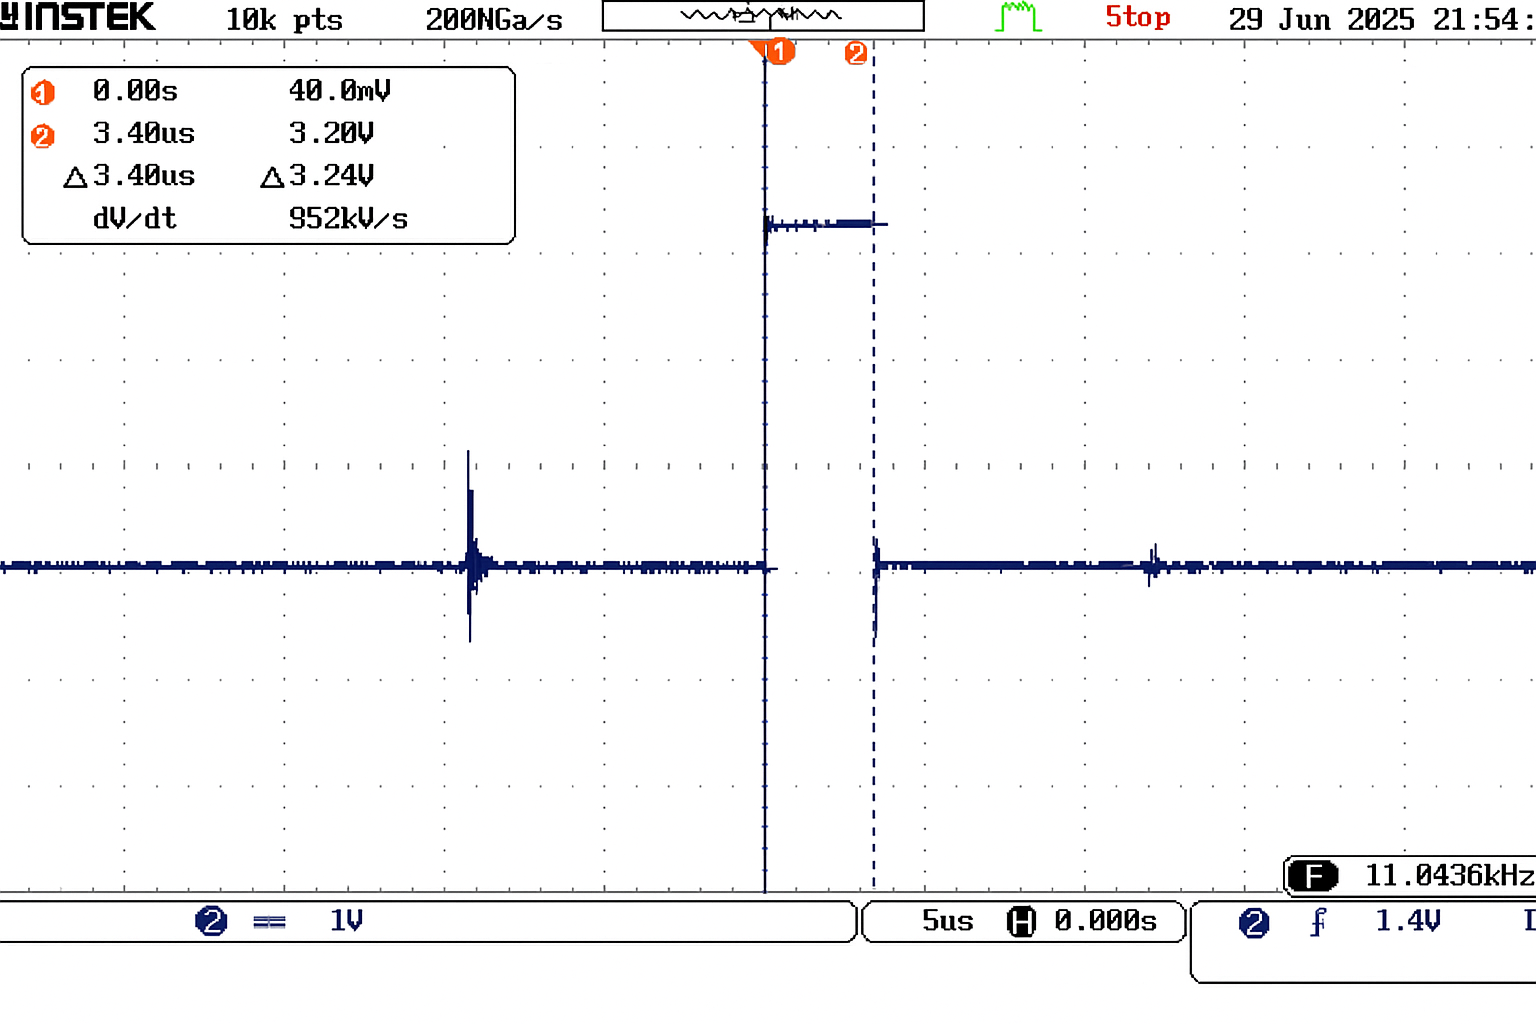
\includegraphics[width=\textwidth]{./CPU_Load_PI}
    \end{minipage}
    \hfill
    \begin{minipage}[b]{0.3\textwidth}
        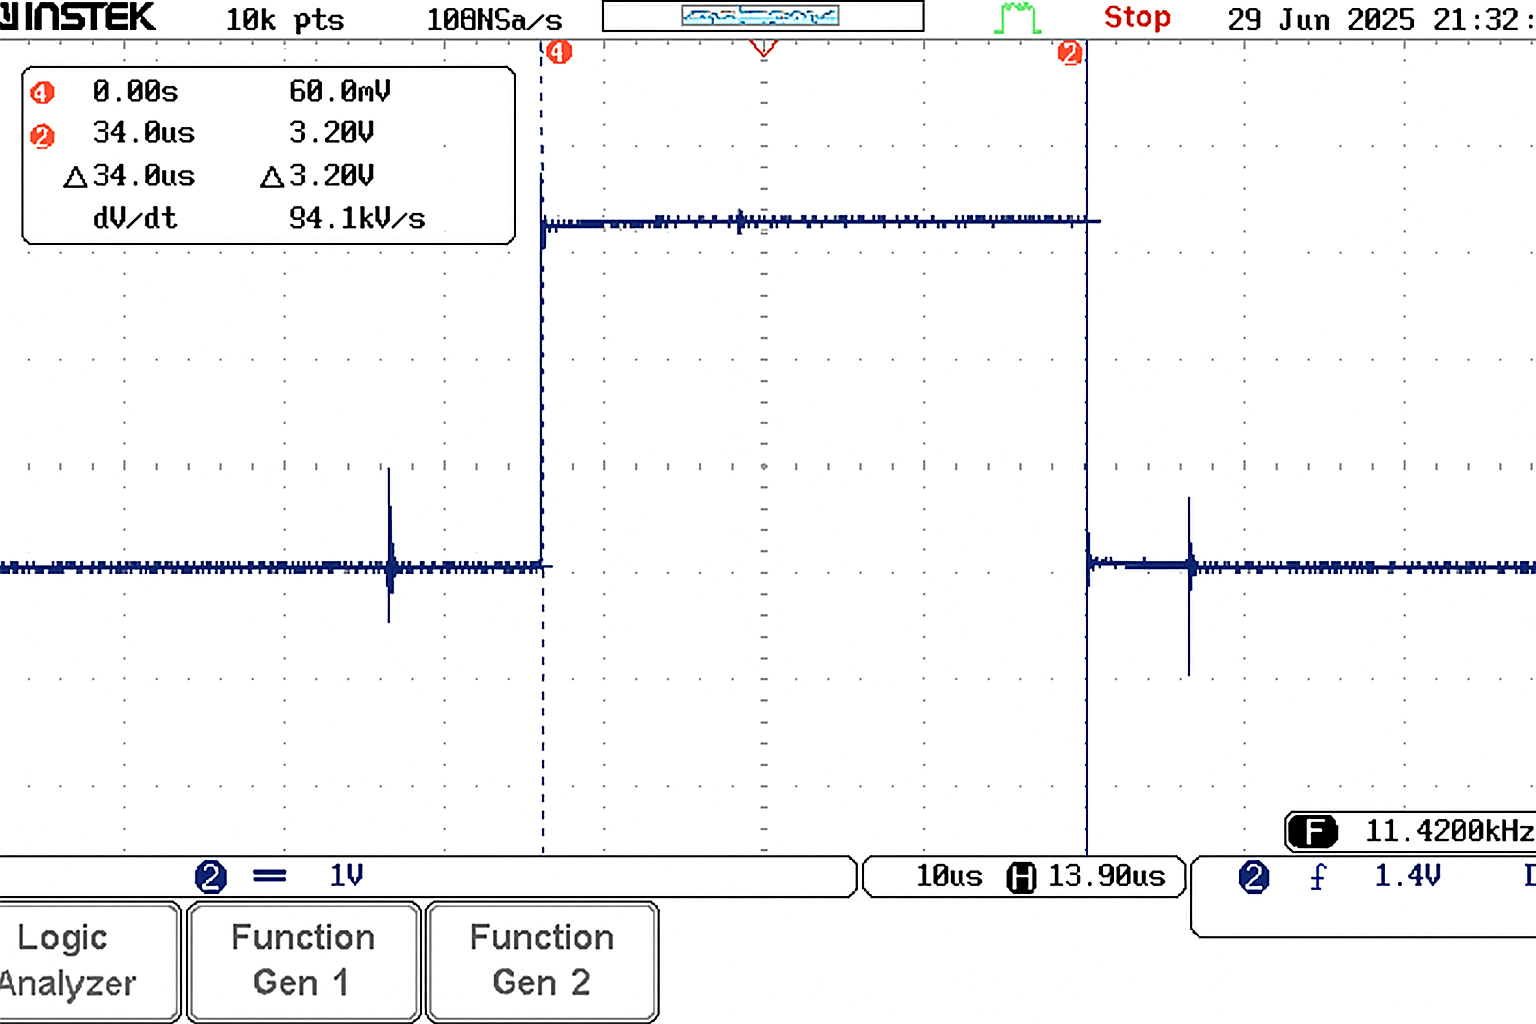
\includegraphics[width=\textwidth]{./CPU_Load_MPC_NHE}
    \end{minipage}
    \hfill
    \begin{minipage}[b]{0.3\textwidth}
        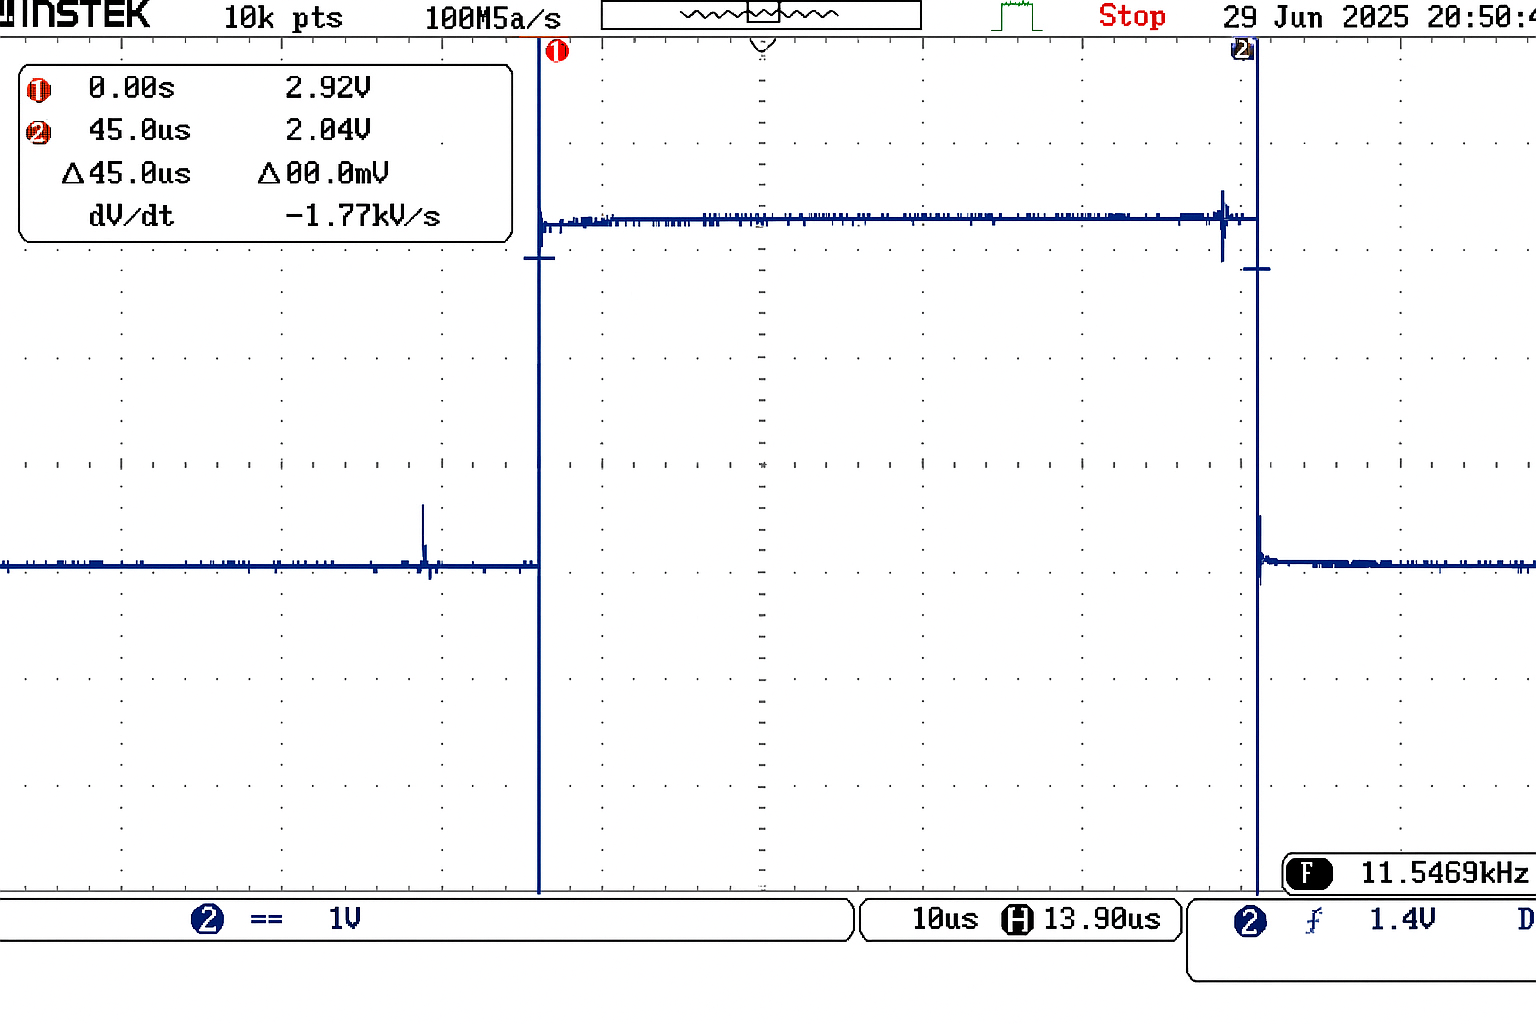
\includegraphics[width=\textwidth]{./CPU_Load_MPC_HE}
    \end{minipage}
    \caption{Experimental results for each controller execution time (a) PI-Controller (b) MMPC, (c) MMPC-HE.}
    \label{fig:minipage_example}
\end{figure}
